\chapter{Arbeitsumgebung}\label{ch:arbeitsumgebung}
In diesem Kapitel ist beschrieben, wie die Arbeitsumgebung des Lernenden während der Probe-IPA aussah.


\section{Arbeitsplatz}\label{sec:arbeitsplatz}
\subsection{Office Arbeitsplatz}\label{subsec:office-arbeitsplatz}
Die Probe-IPA wird am gewohnten Arbeitsplatz im Fünferbüro des Lernenden durchgeführt. Als Arbeitsgerät wird ein Notebook verwendet, welches mithilfe einer Dockingstation das Gerät mit zwei Monitoren und dem Firmennetzwerk verbindet. Der Stuhl und Tisch sind höhenverstellbar, und der Lernende kann dadurch in verschiedenen Sitzpositionen oder stehend arbeiten.

\begin{figure}[H]
    \begin{center}
        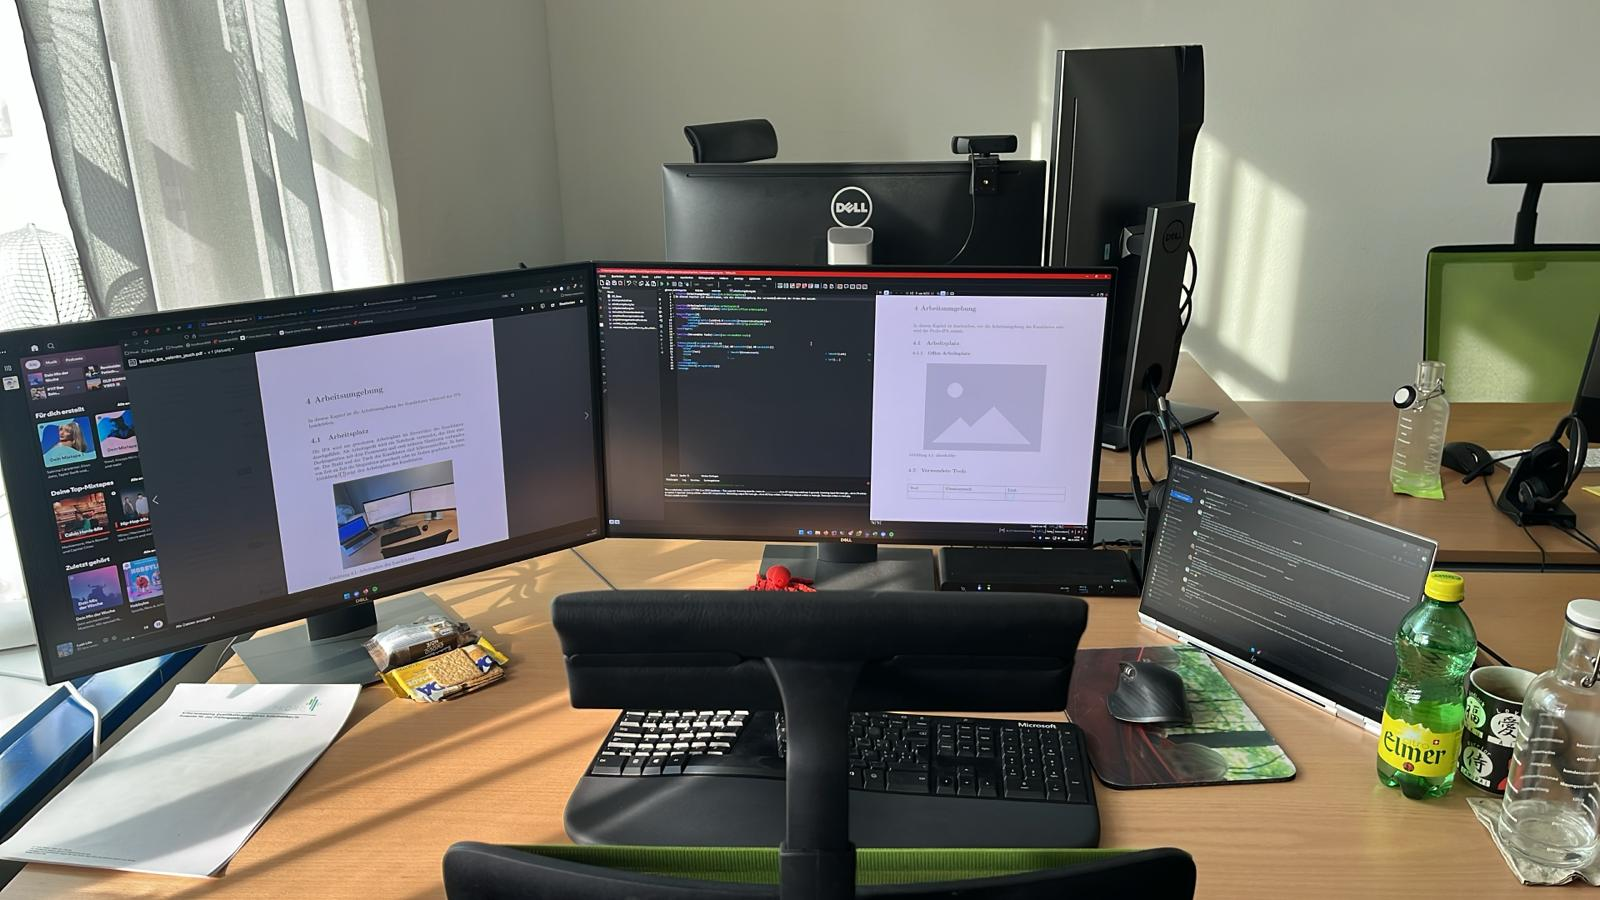
\includegraphics[width=0.8\textwidth]{ressourcen/Arbeitsplatz-Joel-Vontobel}
        \caption[Arbeitsplatz des Lernenden]{Arbeitsplatz des Lernenden}\label{fig:Arbeitsplatz-Joel-Vontobel}
    \end{center}
\end{figure}

\newpage
\section{Verwendete Tools}\label{sec:verwendete-tools}
Die folgende Tabelle zeigt auf, welche Tools für die Umsetzung der Probe-IPA eingesetzt wurden.

\renewcommand{\arraystretch}{1.5}
\begin{longtable}{|p{.22\textwidth}|p{.40\textwidth}|p{.38\textwidth}|}
    \hline
    \textbf{Tool}                    & \textbf{Einsatzzweck}                              & \textbf{Link}                                                             \\ \hline
    IntelliJ                         & Entwicklungsumgebung für die Programmierung        & \url{https://www.jetbrains.com/de-de/idea/}                               \\ \hline
    Docker                           & Ausführen der Programme                            & \url{https://www.docker.com/}                                             \\ \hline
    Git                              & Versionierung vom Quellcode                        & \url{https://git-scm.com/}                                                \\ \hline
    Postman                          & Ausführen von HTTP-Requests (Testen vom Bankend)   & \url{https://www.postman.com/}                                            \\ \hline
    Bitbucket                        & Speicherung der Quellcodes                         & \url{https://bitbucket.org/product/}                                      \\ \hline
    Jenkins                          & Tool für Pipelines um Tests, Codequalität automatisch zu prüfen  & \url{https://www.jenkins.io/}                               \\ \hline
    Confluence                       & Probe-IPA Kriterien                                & \url{https://www.atlassian.com/de/software/confluence}                    \\ \hline
    Jira                             & Aufgabenstellung                                   & \url{https://www.atlassian.com/de/software/jira}                          \\ \hline
    Draw.io                          & Erstellen von Diagrammen und Abbildungen           & \url{https://www.drawio.com/}                                             \\ \hline
    TexStudio                        & Dokumentationstool                                 & \url{https://www.texstudio.org/}                                          \\ \hline
    LaTeX                            & Ein Dokumentenvorbereitungssystem                  & \url{https://www.latex-project.org/}                                      \\ \hline
    Mattermost                       & Text basiertes Kommunikationsmittel                & \url{https://mattermost.com/}                                             \\ \hline
    Microsoft Teams                  & Video basiertes Kommunikationiesmittel             & \url{https://www.microsoft.com/de-ch/microsoft-teams/group-chat-software} \\ \hline
    Microsoft Excel                  & Erstellung und Bearbeitung des Zeitplans           & \url{https://www.microsoft.com/de-ch/microsoft-365/excel?market=ch}       \\ \hline
\end{longtable}
\renewcommand{\arraystretch}{1}
\newpage